\newpage
\section{Auswertung}
\label{sec:Auswertung}
In diesem Abschnitt werden die aufgenommenen Messdaten in Grafiken sowie Tabellen dargestellt und ausgewertet. Grafiken sowie dazugehörige Rechnungen sind mit Python \cite{python} erstellt bzw. berechnet worden.
\subsection{Landé-Faktoren und Kernspins}
\label{sec:kernspin}
In Tabelle (\ref{tab:rf}) sind die aufgenommenen Frequenzen sowie Ströme der Horizontalspule und der Sweepspule für die jeweiligen Transparenzminima eingetragen.
\begin{table}
  \centering
  \caption{RF-Frequenzen und Ströme der Horizonatalspule und Sweepspule.}
  \label{tab:rf}
  \begin{tabular}{c | c | c | c | c}
    \toprule
    $\nu_{RF}$/kHz & $I_{H,87}$/A & $I_{S,87}$/A& $I_{H,85}$/A& $I_{S,85}$/A \\
    \midrule
    100.0 & 0.0 & 0.384 & 0.0 & 0.504 \\
    200.0 & 0.0 & 0.656 & 0.0 & 0.893 \\
    300.0 & 0.012 & 0.467 & 0.012 & 0.896 \\
    400.0 & 0.035 & 0.382 & 0.035 & 0.899 \\
    500.0 & 0.076 & 0.210 & 0.076 & 0.823 \\
    600.0 & 0.102 & 0.134 & 0.102 & 0.792 \\
    700.0 & 0.124 & 0.145 & 0.168 & 0.834 \\
    800.0 & 0.128 & 0.192 & 0.189 & 0.495 \\
    900.0 & 0.146 & 0.220 & 0.197 & 0.401 \\
    1000.0 & 0.169 & 0.200 & 0.231 & 0.262 \\
    \bottomrule
  \end{tabular}
\end{table}
\FloatBarrier
Aus den oben stehenden Strömen wird mit Gleichung (\ref{eqn:bfeld}) das Magnetfeld berechnet:
\begin{equation}
  \label{eqn:bfeld}
  B=\mu_\mathrm{0}\dfrac{8\cdot IN}{\sqrt{125}\cdot R}
\end{equation}
Dabei ist $I$ der Spulenstrom und $\mu_\mathrm{0}$ die magnetische Feldkonstante.
Für die Horizontalspule gilt $N=154$ und $R=\SI{15.69}{\centi\meter}$, für die Sweepspule gilt $N=11$ und $R\SI{16.39}{\centi\meter}$.
Eine lineare Regression des Magnetfeldes der Form $B=a\nu+b$ gegen die eingestellte Frequenz liefert
\begin{align*}
  B_{87} &= \SI{0.156\pm0.007}{\micro\tesla\per\kilo\hertz}\cdot\nu + \SI{1\pm4}{\micro\tesla} \\
  B_{85} &= \SI{0.225\pm0.016}{\micro\tesla\per\kilo\hertz}\cdot\nu + \SI{6\pm10}{\micro\tesla} \\
\end{align*}
Die Daten mit den zugehörigen oben genannten Geraden sind in Abbildung \ref{fig:rf} zu finden:
\begin{figure}[h!]
  \centering
  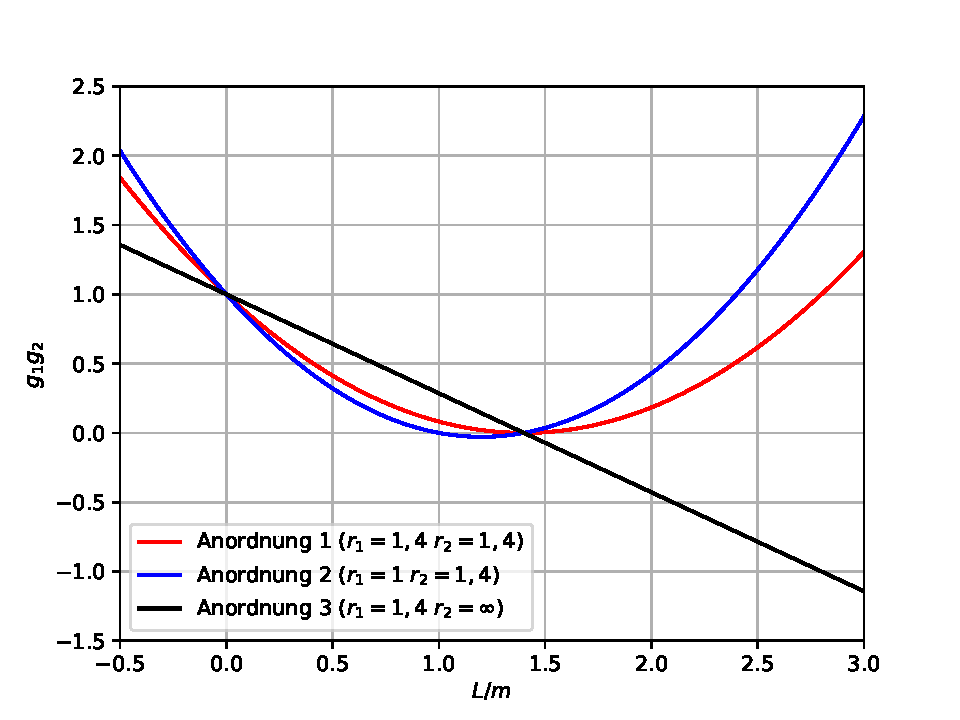
\includegraphics[scale=0.7]{fig/plot1.pdf}
  \caption{Horizontales Magnetfeld gegen die Frequenz.}
  \label{fig:rf}
\end{figure}
\FloatBarrier
Um die Landé-Faktoren zu berechnen wird die Gleichung (\ref{eqn:mf}) wie folgt umgestellt:
\begin{align*}
  h\nu_\mathrm{0}&=g_\mathrm{F}\mu_\mathrm{B}B_\mathrm{0} \\
  \Leftrightarrow \nu_\mathrm{0} &=\dfrac{g_\mathrm{F}\mu_\mathrm{B}B_\mathrm{0}}{h} \\
  \Rightarrow a&=\dfrac{h}{g_\mathrm{F}\mu_\mathrm{B}} \\
  \Leftrightarrow g_\mathrm{F}&=\dfrac{h}{a\mu_\mathrm{B}}
\end{align*}
Mit $h$ als Planckschem Wirkungsquantum und $a$ als Steigung der Geraden aus Abbildung (\ref{fig:rf}).
Damit ergibt sich für die Landé-Faktoren:
\begin{align*}
  g_{\mathrm{F,85}} &= 0.457\pm0.021\\
  g_{\mathrm{F,87}} &= 0.318\pm0.023
\end{align*}
Mit Gleichung \ref{eqn:lande} wird $g_\mathrm{J}$ berechnet.
Mit $S=\dfrac{1}{2}$, $L=0$ und $J=\dfrac{1}{2}$ folgt $g_\mathrm{J} = 2.0023$.
Für die Kernspins gilt
\begin{equation}
  I = \dfrac{g_\mathrm{J}}{2g_\mathrm{F}-\dfrac{1}{2}}
\end{equation}
Damit folgen
\begin{align*}
  I_\mathrm{87} &= 1.69\pm0.10 \\
  I_\mathrm{85} &= 2.65\pm0.23
\end{align*}

\subsection{Isotopenverhältnis}
In Abbildung (\ref{fig:signal}) ist das Signalbild für $\nu=\SI{100}{\kilo\hertz}$ dargestellt.
Aus dem Amplitudenverhältnis der beiden beobachteten Transparenzminima wird das Isotopenverhältnis der untersuchten Probe bestimmt.
\begin{figure}[h!]
  \centering
  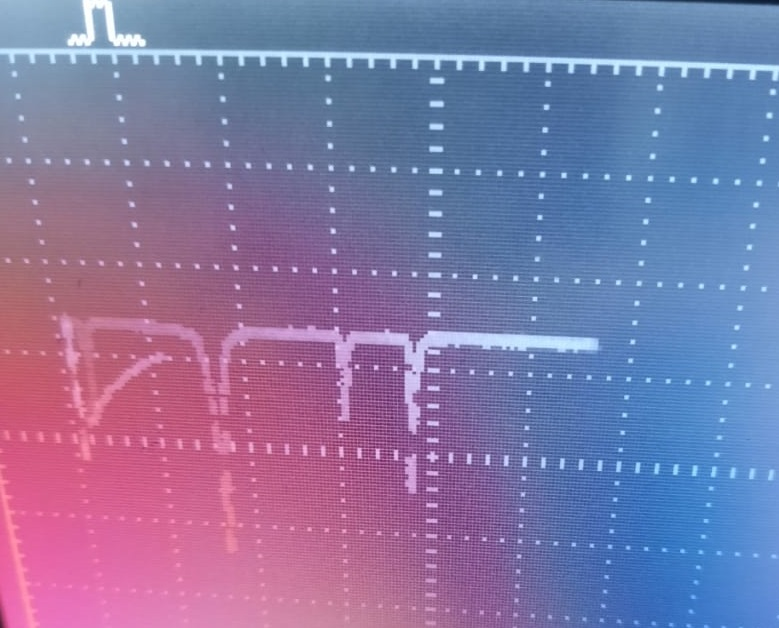
\includegraphics[scale=0.5]{fig/signal.jpg}
  \caption{Oszilloskopbild bei $\SI{100}{\kilo\hertz}$}
  \label{fig:signal}
\end{figure}
Aus diesem Bild werden die Amplituden mit Hilfe von Paint \cite{paint} abgelesen, es ergibt sich für die jeweilige Amplitude:
\begin{align*}
  A_\mathrm{87} &= 77 \, \mathrm{px} \\
  A_\mathrm{85} &= 175 \,\mathrm{px}
\end{align*}
Daraus ergibt sich für die Isotope ein Verhältnis von $^{87}\mathrm{Rb} \approx 31\%$ und $^{85}\mathrm{Rb} \approx 69\%$.
\subsection{Quadratischer Zeeman-Effekt}
Als letztes wird der Einfluss des quadratischen Zeeman-Effekte ausgewertet
Nach Gleichung (\ref{eqn:mf}) für die lineare Näherung und dem quadratischen Teil von Gleichung (\ref{eqn:quadra}) für die quadratische Näherung folgt für die Seemannenergie jeweils:
\begin{align*}
  U_{\mathrm{HF,87,linear}}&= \SI{6.79 \pm 0.31 e-28}{\joule} \\
  U_{\mathrm{HF,85,linear}}&= \SI{6.4 \pm 0.5 e-28}{\joule} \\
  U_{\mathrm{HF,87,quad}}&= \SI{2.29 \pm 0.21 e-31}{\joule} \\
  U_{\mathrm{HF,85,quad}}&= \SI{9.2 \pm 1.3 e-32}{\joule}
\end{align*}
